% Options for packages loaded elsewhere
\PassOptionsToPackage{unicode}{hyperref}
\PassOptionsToPackage{hyphens}{url}
\PassOptionsToPackage{dvipsnames,svgnames,x11names}{xcolor}
%
\documentclass[
  letterpaper,
  DIV=11,
  numbers=noendperiod]{scrartcl}

\usepackage{amsmath,amssymb}
\usepackage{iftex}
\ifPDFTeX
  \usepackage[T1]{fontenc}
  \usepackage[utf8]{inputenc}
  \usepackage{textcomp} % provide euro and other symbols
\else % if luatex or xetex
  \usepackage{unicode-math}
  \defaultfontfeatures{Scale=MatchLowercase}
  \defaultfontfeatures[\rmfamily]{Ligatures=TeX,Scale=1}
\fi
\usepackage{lmodern}
\ifPDFTeX\else  
    % xetex/luatex font selection
\fi
% Use upquote if available, for straight quotes in verbatim environments
\IfFileExists{upquote.sty}{\usepackage{upquote}}{}
\IfFileExists{microtype.sty}{% use microtype if available
  \usepackage[]{microtype}
  \UseMicrotypeSet[protrusion]{basicmath} % disable protrusion for tt fonts
}{}
\makeatletter
\@ifundefined{KOMAClassName}{% if non-KOMA class
  \IfFileExists{parskip.sty}{%
    \usepackage{parskip}
  }{% else
    \setlength{\parindent}{0pt}
    \setlength{\parskip}{6pt plus 2pt minus 1pt}}
}{% if KOMA class
  \KOMAoptions{parskip=half}}
\makeatother
\usepackage{xcolor}
\setlength{\emergencystretch}{3em} % prevent overfull lines
\setcounter{secnumdepth}{-\maxdimen} % remove section numbering
% Make \paragraph and \subparagraph free-standing
\ifx\paragraph\undefined\else
  \let\oldparagraph\paragraph
  \renewcommand{\paragraph}[1]{\oldparagraph{#1}\mbox{}}
\fi
\ifx\subparagraph\undefined\else
  \let\oldsubparagraph\subparagraph
  \renewcommand{\subparagraph}[1]{\oldsubparagraph{#1}\mbox{}}
\fi

\usepackage{color}
\usepackage{fancyvrb}
\newcommand{\VerbBar}{|}
\newcommand{\VERB}{\Verb[commandchars=\\\{\}]}
\DefineVerbatimEnvironment{Highlighting}{Verbatim}{commandchars=\\\{\}}
% Add ',fontsize=\small' for more characters per line
\usepackage{framed}
\definecolor{shadecolor}{RGB}{241,243,245}
\newenvironment{Shaded}{\begin{snugshade}}{\end{snugshade}}
\newcommand{\AlertTok}[1]{\textcolor[rgb]{0.68,0.00,0.00}{#1}}
\newcommand{\AnnotationTok}[1]{\textcolor[rgb]{0.37,0.37,0.37}{#1}}
\newcommand{\AttributeTok}[1]{\textcolor[rgb]{0.40,0.45,0.13}{#1}}
\newcommand{\BaseNTok}[1]{\textcolor[rgb]{0.68,0.00,0.00}{#1}}
\newcommand{\BuiltInTok}[1]{\textcolor[rgb]{0.00,0.23,0.31}{#1}}
\newcommand{\CharTok}[1]{\textcolor[rgb]{0.13,0.47,0.30}{#1}}
\newcommand{\CommentTok}[1]{\textcolor[rgb]{0.37,0.37,0.37}{#1}}
\newcommand{\CommentVarTok}[1]{\textcolor[rgb]{0.37,0.37,0.37}{\textit{#1}}}
\newcommand{\ConstantTok}[1]{\textcolor[rgb]{0.56,0.35,0.01}{#1}}
\newcommand{\ControlFlowTok}[1]{\textcolor[rgb]{0.00,0.23,0.31}{#1}}
\newcommand{\DataTypeTok}[1]{\textcolor[rgb]{0.68,0.00,0.00}{#1}}
\newcommand{\DecValTok}[1]{\textcolor[rgb]{0.68,0.00,0.00}{#1}}
\newcommand{\DocumentationTok}[1]{\textcolor[rgb]{0.37,0.37,0.37}{\textit{#1}}}
\newcommand{\ErrorTok}[1]{\textcolor[rgb]{0.68,0.00,0.00}{#1}}
\newcommand{\ExtensionTok}[1]{\textcolor[rgb]{0.00,0.23,0.31}{#1}}
\newcommand{\FloatTok}[1]{\textcolor[rgb]{0.68,0.00,0.00}{#1}}
\newcommand{\FunctionTok}[1]{\textcolor[rgb]{0.28,0.35,0.67}{#1}}
\newcommand{\ImportTok}[1]{\textcolor[rgb]{0.00,0.46,0.62}{#1}}
\newcommand{\InformationTok}[1]{\textcolor[rgb]{0.37,0.37,0.37}{#1}}
\newcommand{\KeywordTok}[1]{\textcolor[rgb]{0.00,0.23,0.31}{#1}}
\newcommand{\NormalTok}[1]{\textcolor[rgb]{0.00,0.23,0.31}{#1}}
\newcommand{\OperatorTok}[1]{\textcolor[rgb]{0.37,0.37,0.37}{#1}}
\newcommand{\OtherTok}[1]{\textcolor[rgb]{0.00,0.23,0.31}{#1}}
\newcommand{\PreprocessorTok}[1]{\textcolor[rgb]{0.68,0.00,0.00}{#1}}
\newcommand{\RegionMarkerTok}[1]{\textcolor[rgb]{0.00,0.23,0.31}{#1}}
\newcommand{\SpecialCharTok}[1]{\textcolor[rgb]{0.37,0.37,0.37}{#1}}
\newcommand{\SpecialStringTok}[1]{\textcolor[rgb]{0.13,0.47,0.30}{#1}}
\newcommand{\StringTok}[1]{\textcolor[rgb]{0.13,0.47,0.30}{#1}}
\newcommand{\VariableTok}[1]{\textcolor[rgb]{0.07,0.07,0.07}{#1}}
\newcommand{\VerbatimStringTok}[1]{\textcolor[rgb]{0.13,0.47,0.30}{#1}}
\newcommand{\WarningTok}[1]{\textcolor[rgb]{0.37,0.37,0.37}{\textit{#1}}}

\providecommand{\tightlist}{%
  \setlength{\itemsep}{0pt}\setlength{\parskip}{0pt}}\usepackage{longtable,booktabs,array}
\usepackage{calc} % for calculating minipage widths
% Correct order of tables after \paragraph or \subparagraph
\usepackage{etoolbox}
\makeatletter
\patchcmd\longtable{\par}{\if@noskipsec\mbox{}\fi\par}{}{}
\makeatother
% Allow footnotes in longtable head/foot
\IfFileExists{footnotehyper.sty}{\usepackage{footnotehyper}}{\usepackage{footnote}}
\makesavenoteenv{longtable}
\usepackage{graphicx}
\makeatletter
\def\maxwidth{\ifdim\Gin@nat@width>\linewidth\linewidth\else\Gin@nat@width\fi}
\def\maxheight{\ifdim\Gin@nat@height>\textheight\textheight\else\Gin@nat@height\fi}
\makeatother
% Scale images if necessary, so that they will not overflow the page
% margins by default, and it is still possible to overwrite the defaults
% using explicit options in \includegraphics[width, height, ...]{}
\setkeys{Gin}{width=\maxwidth,height=\maxheight,keepaspectratio}
% Set default figure placement to htbp
\makeatletter
\def\fps@figure{htbp}
\makeatother

\KOMAoption{captions}{tableheading}
\makeatletter
\makeatother
\makeatletter
\makeatother
\makeatletter
\@ifpackageloaded{caption}{}{\usepackage{caption}}
\AtBeginDocument{%
\ifdefined\contentsname
  \renewcommand*\contentsname{Table of contents}
\else
  \newcommand\contentsname{Table of contents}
\fi
\ifdefined\listfigurename
  \renewcommand*\listfigurename{List of Figures}
\else
  \newcommand\listfigurename{List of Figures}
\fi
\ifdefined\listtablename
  \renewcommand*\listtablename{List of Tables}
\else
  \newcommand\listtablename{List of Tables}
\fi
\ifdefined\figurename
  \renewcommand*\figurename{Figure}
\else
  \newcommand\figurename{Figure}
\fi
\ifdefined\tablename
  \renewcommand*\tablename{Table}
\else
  \newcommand\tablename{Table}
\fi
}
\@ifpackageloaded{float}{}{\usepackage{float}}
\floatstyle{ruled}
\@ifundefined{c@chapter}{\newfloat{codelisting}{h}{lop}}{\newfloat{codelisting}{h}{lop}[chapter]}
\floatname{codelisting}{Listing}
\newcommand*\listoflistings{\listof{codelisting}{List of Listings}}
\makeatother
\makeatletter
\@ifpackageloaded{caption}{}{\usepackage{caption}}
\@ifpackageloaded{subcaption}{}{\usepackage{subcaption}}
\makeatother
\makeatletter
\@ifpackageloaded{tcolorbox}{}{\usepackage[skins,breakable]{tcolorbox}}
\makeatother
\makeatletter
\@ifundefined{shadecolor}{\definecolor{shadecolor}{rgb}{.97, .97, .97}}
\makeatother
\makeatletter
\makeatother
\makeatletter
\makeatother
\ifLuaTeX
  \usepackage{selnolig}  % disable illegal ligatures
\fi
\IfFileExists{bookmark.sty}{\usepackage{bookmark}}{\usepackage{hyperref}}
\IfFileExists{xurl.sty}{\usepackage{xurl}}{} % add URL line breaks if available
\urlstyle{same} % disable monospaced font for URLs
\hypersetup{
  pdftitle={class10 structural bioinformatics p1},
  pdfauthor={amy (pid A16962111)},
  colorlinks=true,
  linkcolor={blue},
  filecolor={Maroon},
  citecolor={Blue},
  urlcolor={Blue},
  pdfcreator={LaTeX via pandoc}}

\title{class10 structural bioinformatics p1}
\author{amy (pid A16962111)}
\date{}

\begin{document}
\maketitle
\ifdefined\Shaded\renewenvironment{Shaded}{\begin{tcolorbox}[boxrule=0pt, interior hidden, borderline west={3pt}{0pt}{shadecolor}, enhanced, sharp corners, breakable, frame hidden]}{\end{tcolorbox}}\fi

\hypertarget{the-pdb-database}{%
\section{the PDB database}\label{the-pdb-database}}

Here we examine the size and composition of the main database of
biomolecular structures - the PDB.

Get a CSV file from the PDB database and read it into R.

\begin{Shaded}
\begin{Highlighting}[]
\NormalTok{pdbstats }\OtherTok{\textless{}{-}} \FunctionTok{read.csv}\NormalTok{(}\StringTok{"Data Export Summary.csv"}\NormalTok{, }\AttributeTok{row.names=}\DecValTok{1}\NormalTok{)}
\NormalTok{pdbstats}
\end{Highlighting}
\end{Shaded}

\begin{verbatim}
                          X.ray     EM    NMR Multiple.methods Neutron Other
Protein (only)          161,663 12,592 12,337              200      74    32
Protein/Oligosaccharide   9,348  2,167     34                8       2     0
Protein/NA                8,404  3,924    286                7       0     0
Nucleic acid (only)       2,758    125  1,477               14       3     1
Other                       164      9     33                0       0     0
Oligosaccharide (only)       11      0      6                1       0     4
                          Total
Protein (only)          186,898
Protein/Oligosaccharide  11,559
Protein/NA               12,621
Nucleic acid (only)       4,378
Other                       206
Oligosaccharide (only)       22
\end{verbatim}

\begin{itemize}
\item
  \textbf{Q1:}~What percentage of structures in the PDB are solved by
  X-Ray and Electron Microscopy.

  My pbdstats dataframe has numbers with commas in them. This may cause
  us problems.

\begin{Shaded}
\begin{Highlighting}[]
\FunctionTok{sum}\NormalTok{(}\FunctionTok{as.numeric}\NormalTok{(pdbstats}\SpecialCharTok{$}\NormalTok{X.ray, pdbstats}\SpecialCharTok{$}\NormalTok{EM))}
\end{Highlighting}
\end{Shaded}

\begin{verbatim}
Warning: NAs introduced by coercion
\end{verbatim}

\begin{verbatim}
[1] NA
\end{verbatim}

  We found a function called \texttt{gsub()} . I can use this to make a
  function that I can use for every column in the table.

\begin{Shaded}
\begin{Highlighting}[]
\NormalTok{commasum }\OtherTok{\textless{}{-}} \ControlFlowTok{function}\NormalTok{(x) \{}
  \FunctionTok{sum}\NormalTok{(}\FunctionTok{as.numeric}\NormalTok{(}\FunctionTok{gsub}\NormalTok{(}\StringTok{","}\NormalTok{, }\StringTok{""}\NormalTok{, x)))}
\NormalTok{\}}

\NormalTok{totals }\OtherTok{\textless{}{-}} \FunctionTok{apply}\NormalTok{(pdbstats, }\DecValTok{2}\NormalTok{, commasum)}
\NormalTok{totals}
\end{Highlighting}
\end{Shaded}

\begin{verbatim}
           X.ray               EM              NMR Multiple.methods 
          182348            18817            14173              230 
         Neutron            Other            Total 
              79               37           215684 
\end{verbatim}

\begin{Shaded}
\begin{Highlighting}[]
\FunctionTok{round}\NormalTok{(totals}\SpecialCharTok{/}\NormalTok{totals[}\StringTok{"Total"}\NormalTok{]}\SpecialCharTok{*}\DecValTok{100}\NormalTok{, }\DecValTok{2}\NormalTok{)}
\end{Highlighting}
\end{Shaded}

\begin{verbatim}
           X.ray               EM              NMR Multiple.methods 
           84.54             8.72             6.57             0.11 
         Neutron            Other            Total 
            0.04             0.02           100.00 
\end{verbatim}

  85\% were solved by x-ray and 9\% by EM.
\item
  \textbf{Q2:}~What proportion of structures in the PDB are protein?

\begin{Shaded}
\begin{Highlighting}[]
\FunctionTok{commasum}\NormalTok{(pdbstats[}\StringTok{"Protein (only)"}\NormalTok{, }\StringTok{"Total"}\NormalTok{])}\SpecialCharTok{/}\NormalTok{totals[}\StringTok{"Total"}\NormalTok{]}\SpecialCharTok{*}\DecValTok{100}
\end{Highlighting}
\end{Shaded}

\begin{verbatim}
   Total 
86.65362 
\end{verbatim}

  87\%
\item
  \textbf{Q.} What fraction of Uniprot structures are represented in the
  PDB?

  0.09\%
\end{itemize}

\begin{Shaded}
\begin{Highlighting}[]
\DecValTok{215684}\SpecialCharTok{/}\DecValTok{249751891}\SpecialCharTok{*}\DecValTok{100}
\end{Highlighting}
\end{Shaded}

\begin{verbatim}
[1] 0.08635931
\end{verbatim}

\hypertarget{visualizing-protein-structure}{%
\section{visualizing protein
structure}\label{visualizing-protein-structure}}

We will learn the basics of Mol* (mol-star) homepage:
\url{https://molstar.org/viewer/}

We will play with PDB 1HSG:

\begin{figure}

{\centering 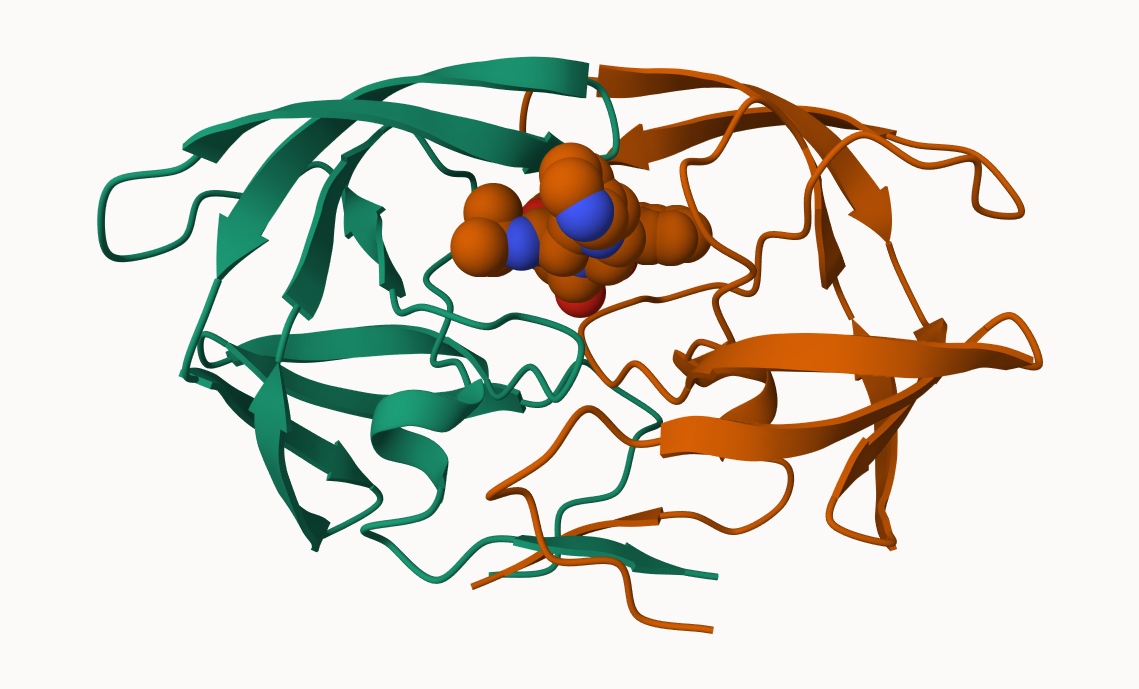
\includegraphics{1HSG.png}

}

\caption{HIV-Pr with a bound inhibitor}

\end{figure}

\begin{figure}

{\centering 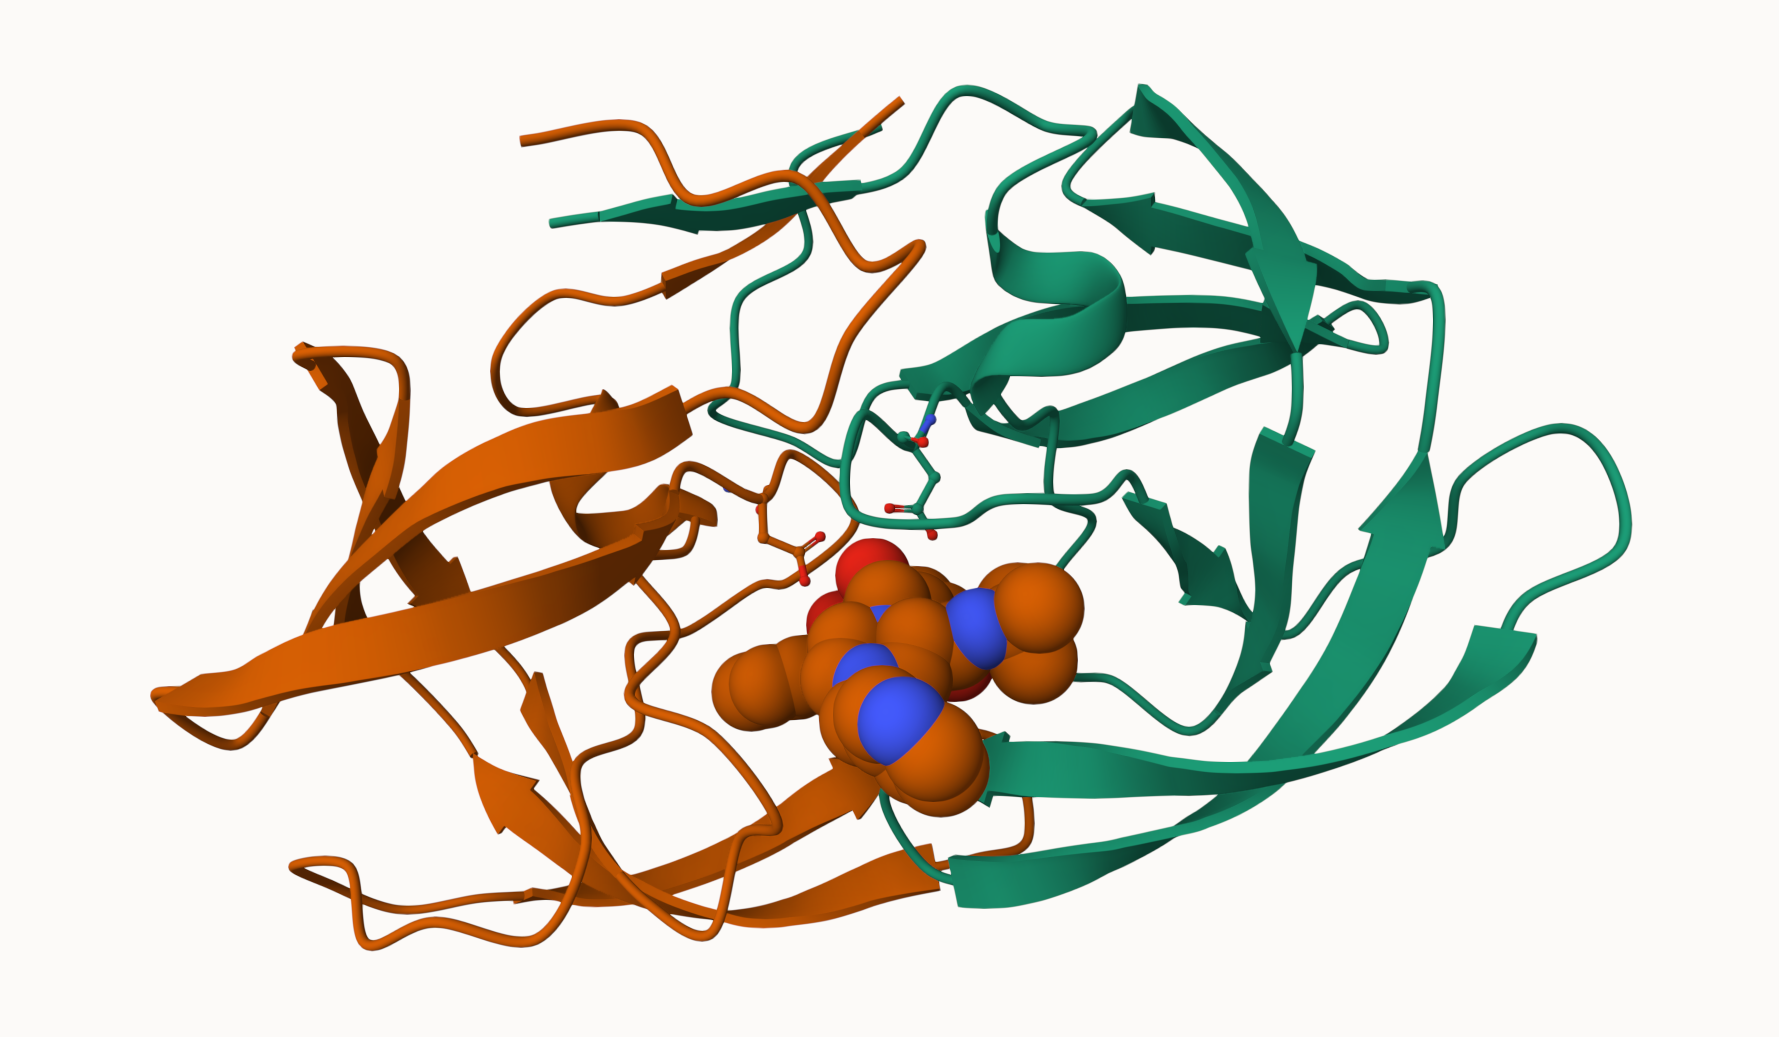
\includegraphics{1HSG copy.png}

}

\caption{with ASP25 residues represented as ball-and-stick figures}

\end{figure}

\hypertarget{back-to-r-and-working-with-pdb-structures}{%
\subsection{back to R and working with PDB
structures}\label{back-to-r-and-working-with-pdb-structures}}

\begin{Shaded}
\begin{Highlighting}[]
\FunctionTok{library}\NormalTok{(bio3d)}
\NormalTok{hiv }\OtherTok{\textless{}{-}} \FunctionTok{read.pdb}\NormalTok{(}\StringTok{"1hsg"}\NormalTok{)}
\end{Highlighting}
\end{Shaded}

\begin{verbatim}
  Note: Accessing on-line PDB file
\end{verbatim}

\begin{Shaded}
\begin{Highlighting}[]
\NormalTok{hiv}
\end{Highlighting}
\end{Shaded}

\begin{verbatim}

 Call:  read.pdb(file = "1hsg")

   Total Models#: 1
     Total Atoms#: 1686,  XYZs#: 5058  Chains#: 2  (values: A B)

     Protein Atoms#: 1514  (residues/Calpha atoms#: 198)
     Nucleic acid Atoms#: 0  (residues/phosphate atoms#: 0)

     Non-protein/nucleic Atoms#: 172  (residues: 128)
     Non-protein/nucleic resid values: [ HOH (127), MK1 (1) ]

   Protein sequence:
      PQITLWQRPLVTIKIGGQLKEALLDTGADDTVLEEMSLPGRWKPKMIGGIGGFIKVRQYD
      QILIEICGHKAIGTVLVGPTPVNIIGRNLLTQIGCTLNFPQITLWQRPLVTIKIGGQLKE
      ALLDTGADDTVLEEMSLPGRWKPKMIGGIGGFIKVRQYDQILIEICGHKAIGTVLVGPTP
      VNIIGRNLLTQIGCTLNF

+ attr: atom, xyz, seqres, helix, sheet,
        calpha, remark, call
\end{verbatim}

\begin{Shaded}
\begin{Highlighting}[]
\FunctionTok{head}\NormalTok{(hiv}\SpecialCharTok{$}\NormalTok{atom)}
\end{Highlighting}
\end{Shaded}

\begin{verbatim}
  type eleno elety  alt resid chain resno insert      x      y     z o     b
1 ATOM     1     N <NA>   PRO     A     1   <NA> 29.361 39.686 5.862 1 38.10
2 ATOM     2    CA <NA>   PRO     A     1   <NA> 30.307 38.663 5.319 1 40.62
3 ATOM     3     C <NA>   PRO     A     1   <NA> 29.760 38.071 4.022 1 42.64
4 ATOM     4     O <NA>   PRO     A     1   <NA> 28.600 38.302 3.676 1 43.40
5 ATOM     5    CB <NA>   PRO     A     1   <NA> 30.508 37.541 6.342 1 37.87
6 ATOM     6    CG <NA>   PRO     A     1   <NA> 29.296 37.591 7.162 1 38.40
  segid elesy charge
1  <NA>     N   <NA>
2  <NA>     C   <NA>
3  <NA>     C   <NA>
4  <NA>     O   <NA>
5  <NA>     C   <NA>
6  <NA>     C   <NA>
\end{verbatim}

\begin{Shaded}
\begin{Highlighting}[]
\FunctionTok{pdbseq}\NormalTok{(hiv)}
\end{Highlighting}
\end{Shaded}

\begin{verbatim}
  1   2   3   4   5   6   7   8   9  10  11  12  13  14  15  16  17  18  19  20 
"P" "Q" "I" "T" "L" "W" "Q" "R" "P" "L" "V" "T" "I" "K" "I" "G" "G" "Q" "L" "K" 
 21  22  23  24  25  26  27  28  29  30  31  32  33  34  35  36  37  38  39  40 
"E" "A" "L" "L" "D" "T" "G" "A" "D" "D" "T" "V" "L" "E" "E" "M" "S" "L" "P" "G" 
 41  42  43  44  45  46  47  48  49  50  51  52  53  54  55  56  57  58  59  60 
"R" "W" "K" "P" "K" "M" "I" "G" "G" "I" "G" "G" "F" "I" "K" "V" "R" "Q" "Y" "D" 
 61  62  63  64  65  66  67  68  69  70  71  72  73  74  75  76  77  78  79  80 
"Q" "I" "L" "I" "E" "I" "C" "G" "H" "K" "A" "I" "G" "T" "V" "L" "V" "G" "P" "T" 
 81  82  83  84  85  86  87  88  89  90  91  92  93  94  95  96  97  98  99   1 
"P" "V" "N" "I" "I" "G" "R" "N" "L" "L" "T" "Q" "I" "G" "C" "T" "L" "N" "F" "P" 
  2   3   4   5   6   7   8   9  10  11  12  13  14  15  16  17  18  19  20  21 
"Q" "I" "T" "L" "W" "Q" "R" "P" "L" "V" "T" "I" "K" "I" "G" "G" "Q" "L" "K" "E" 
 22  23  24  25  26  27  28  29  30  31  32  33  34  35  36  37  38  39  40  41 
"A" "L" "L" "D" "T" "G" "A" "D" "D" "T" "V" "L" "E" "E" "M" "S" "L" "P" "G" "R" 
 42  43  44  45  46  47  48  49  50  51  52  53  54  55  56  57  58  59  60  61 
"W" "K" "P" "K" "M" "I" "G" "G" "I" "G" "G" "F" "I" "K" "V" "R" "Q" "Y" "D" "Q" 
 62  63  64  65  66  67  68  69  70  71  72  73  74  75  76  77  78  79  80  81 
"I" "L" "I" "E" "I" "C" "G" "H" "K" "A" "I" "G" "T" "V" "L" "V" "G" "P" "T" "P" 
 82  83  84  85  86  87  88  89  90  91  92  93  94  95  96  97  98  99 
"V" "N" "I" "I" "G" "R" "N" "L" "L" "T" "Q" "I" "G" "C" "T" "L" "N" "F" 
\end{verbatim}

here we will do a normal mode analysis (NMA) to predict functional
motions of a kinase protein

\begin{Shaded}
\begin{Highlighting}[]
\NormalTok{adk }\OtherTok{\textless{}{-}} \FunctionTok{read.pdb}\NormalTok{(}\StringTok{"6s36"}\NormalTok{)}
\end{Highlighting}
\end{Shaded}

\begin{verbatim}
  Note: Accessing on-line PDB file
   PDB has ALT records, taking A only, rm.alt=TRUE
\end{verbatim}

\begin{Shaded}
\begin{Highlighting}[]
\NormalTok{adk}
\end{Highlighting}
\end{Shaded}

\begin{verbatim}

 Call:  read.pdb(file = "6s36")

   Total Models#: 1
     Total Atoms#: 1898,  XYZs#: 5694  Chains#: 1  (values: A)

     Protein Atoms#: 1654  (residues/Calpha atoms#: 214)
     Nucleic acid Atoms#: 0  (residues/phosphate atoms#: 0)

     Non-protein/nucleic Atoms#: 244  (residues: 244)
     Non-protein/nucleic resid values: [ CL (3), HOH (238), MG (2), NA (1) ]

   Protein sequence:
      MRIILLGAPGAGKGTQAQFIMEKYGIPQISTGDMLRAAVKSGSELGKQAKDIMDAGKLVT
      DELVIALVKERIAQEDCRNGFLLDGFPRTIPQADAMKEAGINVDYVLEFDVPDELIVDKI
      VGRRVHAPSGRVYHVKFNPPKVEGKDDVTGEELTTRKDDQEETVRKRLVEYHQMTAPLIG
      YYSKEAEAGNTKYAKVDGTKPVAEVRADLEKILG

+ attr: atom, xyz, seqres, helix, sheet,
        calpha, remark, call
\end{verbatim}

\begin{Shaded}
\begin{Highlighting}[]
\NormalTok{modes }\OtherTok{\textless{}{-}} \FunctionTok{nma}\NormalTok{(adk)}
\end{Highlighting}
\end{Shaded}

\begin{verbatim}
 Building Hessian...        Done in 0.046 seconds.
 Diagonalizing Hessian...   Done in 0.526 seconds.
\end{verbatim}

\begin{Shaded}
\begin{Highlighting}[]
\FunctionTok{plot}\NormalTok{(modes)}
\end{Highlighting}
\end{Shaded}

\begin{figure}[H]

{\centering 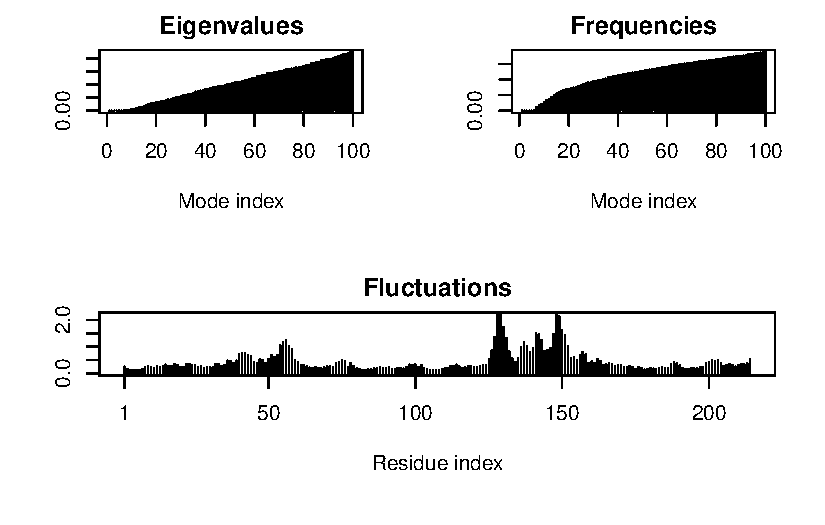
\includegraphics{class10_files/figure-pdf/unnamed-chunk-11-1.pdf}

}

\end{figure}

Make a ``movie'' called a trajectory of predicted motions.

\begin{Shaded}
\begin{Highlighting}[]
\FunctionTok{mktrj}\NormalTok{(modes, }\AttributeTok{file=}\StringTok{"adk\_m7.pdb"}\NormalTok{)}
\end{Highlighting}
\end{Shaded}

Then I can open this file in Mol*

\includegraphics{ADK_M7.PDB_animate-trajectory.mp4}



\end{document}
